\documentclass[11pt,a4paper]{ctexart}
\usepackage[margin=2.3cm]{geometry}
\usepackage{graphicx}
\usepackage{booktabs}
\usepackage{amsmath,amssymb}
\usepackage{array}
\usepackage[table]{xcolor}
\usepackage{caption}
\captionsetup{font=small,labelfont=bf}
\usepackage[colorlinks=true,linkcolor=blue!55!black,citecolor=blue!55!black,urlcolor=blue!55!black]{hyperref}
\setlength{\parskip}{2pt}
\graphicspath{{figures/}}
\newcommand{\up}{$_{\uparrow}$}
\newcommand{\dn}{$_{\downarrow}$}

\title{交通视频短时预判软件\\\large 技术报告}
\author{参赛团队}
\date{}

\begin{document}
\maketitle
\vspace{-1.4em}

\section{作品概述}

\textbf{作品定位。}本作品是一套可直接运行的交通视频短时预判软件：输入
2$\sim$30 秒单目视频，选择 0.1、0.5、1、2 秒四个预判梯度之一，输出一段
\emph{带目标类型与预判位置的连续视频}，同时生成一份机器可读的逐梯度精度报告。
系统全部过程因果——每一帧的预判只使用当前帧及其之前的信息，不使用任何未来帧。

\textbf{要解决的现实问题。}路口与园区已装监控相机数量巨大，但它们只能"看到现在"。
运维方真正需要的是"下一步在哪"：车辆是否会越过停止线、行人是否会进入车道、
骑行者是否会突然变道。给每个机位加装雷达或激光雷达在成本上不成立，而纯视觉方案
往往被当成"跟踪任务"做完就停，不交付预判，也不说明预判在什么范围内可信。

\textbf{目标用户与应用场景}（待与需求方最终确认）：交通管理部门的路口与路段监控
（短时冲突预警）、园区与校园安保（重点区域目标趋势提示）、以及视频监控集成商
（作为算法模块嵌入既有平台）。三类用户的共同点是：只有单目相机、机位固定、
不接受额外硬件成本。

\textbf{本作品交付了什么。}
(1) 可运行的软件与命令行接口；
(2) 四个预判梯度上完整、可复现的实测精度；
(3) 一份对\emph{误差结构}的刻画——误差长什么样、错在哪一侧、哪些改进方向已经证否；
(4) 全部源码、评测脚本与标注工具以 AGPL-3.0 开放，并公开 12 条技术路线的负结果。

\textbf{一句话概括本作品的主张：}在短时、单目、无标定的设定下，
预判精度的瓶颈不在运动模型的复杂程度，而在身份关联的稳定性、固定场景结构的处理，
以及对误差分布的正确认识。本报告用实测数据支撑这一主张。

\section{需求分析与总体方案}

\subsection{需求分解}

把"输入一段视频、输出预判"拆开，任一环失效都会污染最终结果，因此六环都要单独设防：

\begin{enumerate}\setlength{\itemsep}{1pt}
  \item \textbf{检测}：在 1280 分辨率下稳定检出车、卡车、公交、非机动车、行人、
        标志牌、路桩等目标；
  \item \textbf{跟踪与关联}：维持稳定的目标身份，不让串轨把速度估计带偏；
  \item \textbf{运动状态判定}：区分"在动"与"没动"——停放车辆不应被赋予速度，
        固定结构不应时隐时现；
  \item \textbf{运动估计}：由当前帧及历史因果地估计速度；
  \item \textbf{梯度外推}：在四个时间梯度上给出预判位置，并标注可信度；
  \item \textbf{评测与呈现}：输出可核验的逐梯度精度，而不是只给一段好看的视频。
\end{enumerate}

该分解直接来自误差归因：实测显示 7.8\% 的样本（串轨样本）贡献了 26\% 的误差总量，
而遮挡断档样本的误差与连续样本几乎相同——即误差主要来自关联层与状态层，
不是运动模型的复杂度。

\subsection{总体方案}

系统的总体架构如图~\ref{fig:arch}。主链路是"检测 $\rightarrow$ 关联 $\rightarrow$
状态机 $\rightarrow$ 运动估计 $\rightarrow$ 四梯度外推 $\rightarrow$ 渲染"；
静态结构作为独立支路并行处理，其确认结果注入渲染层；输出为视频与精度报告两件。

\begin{figure}[t]\centering
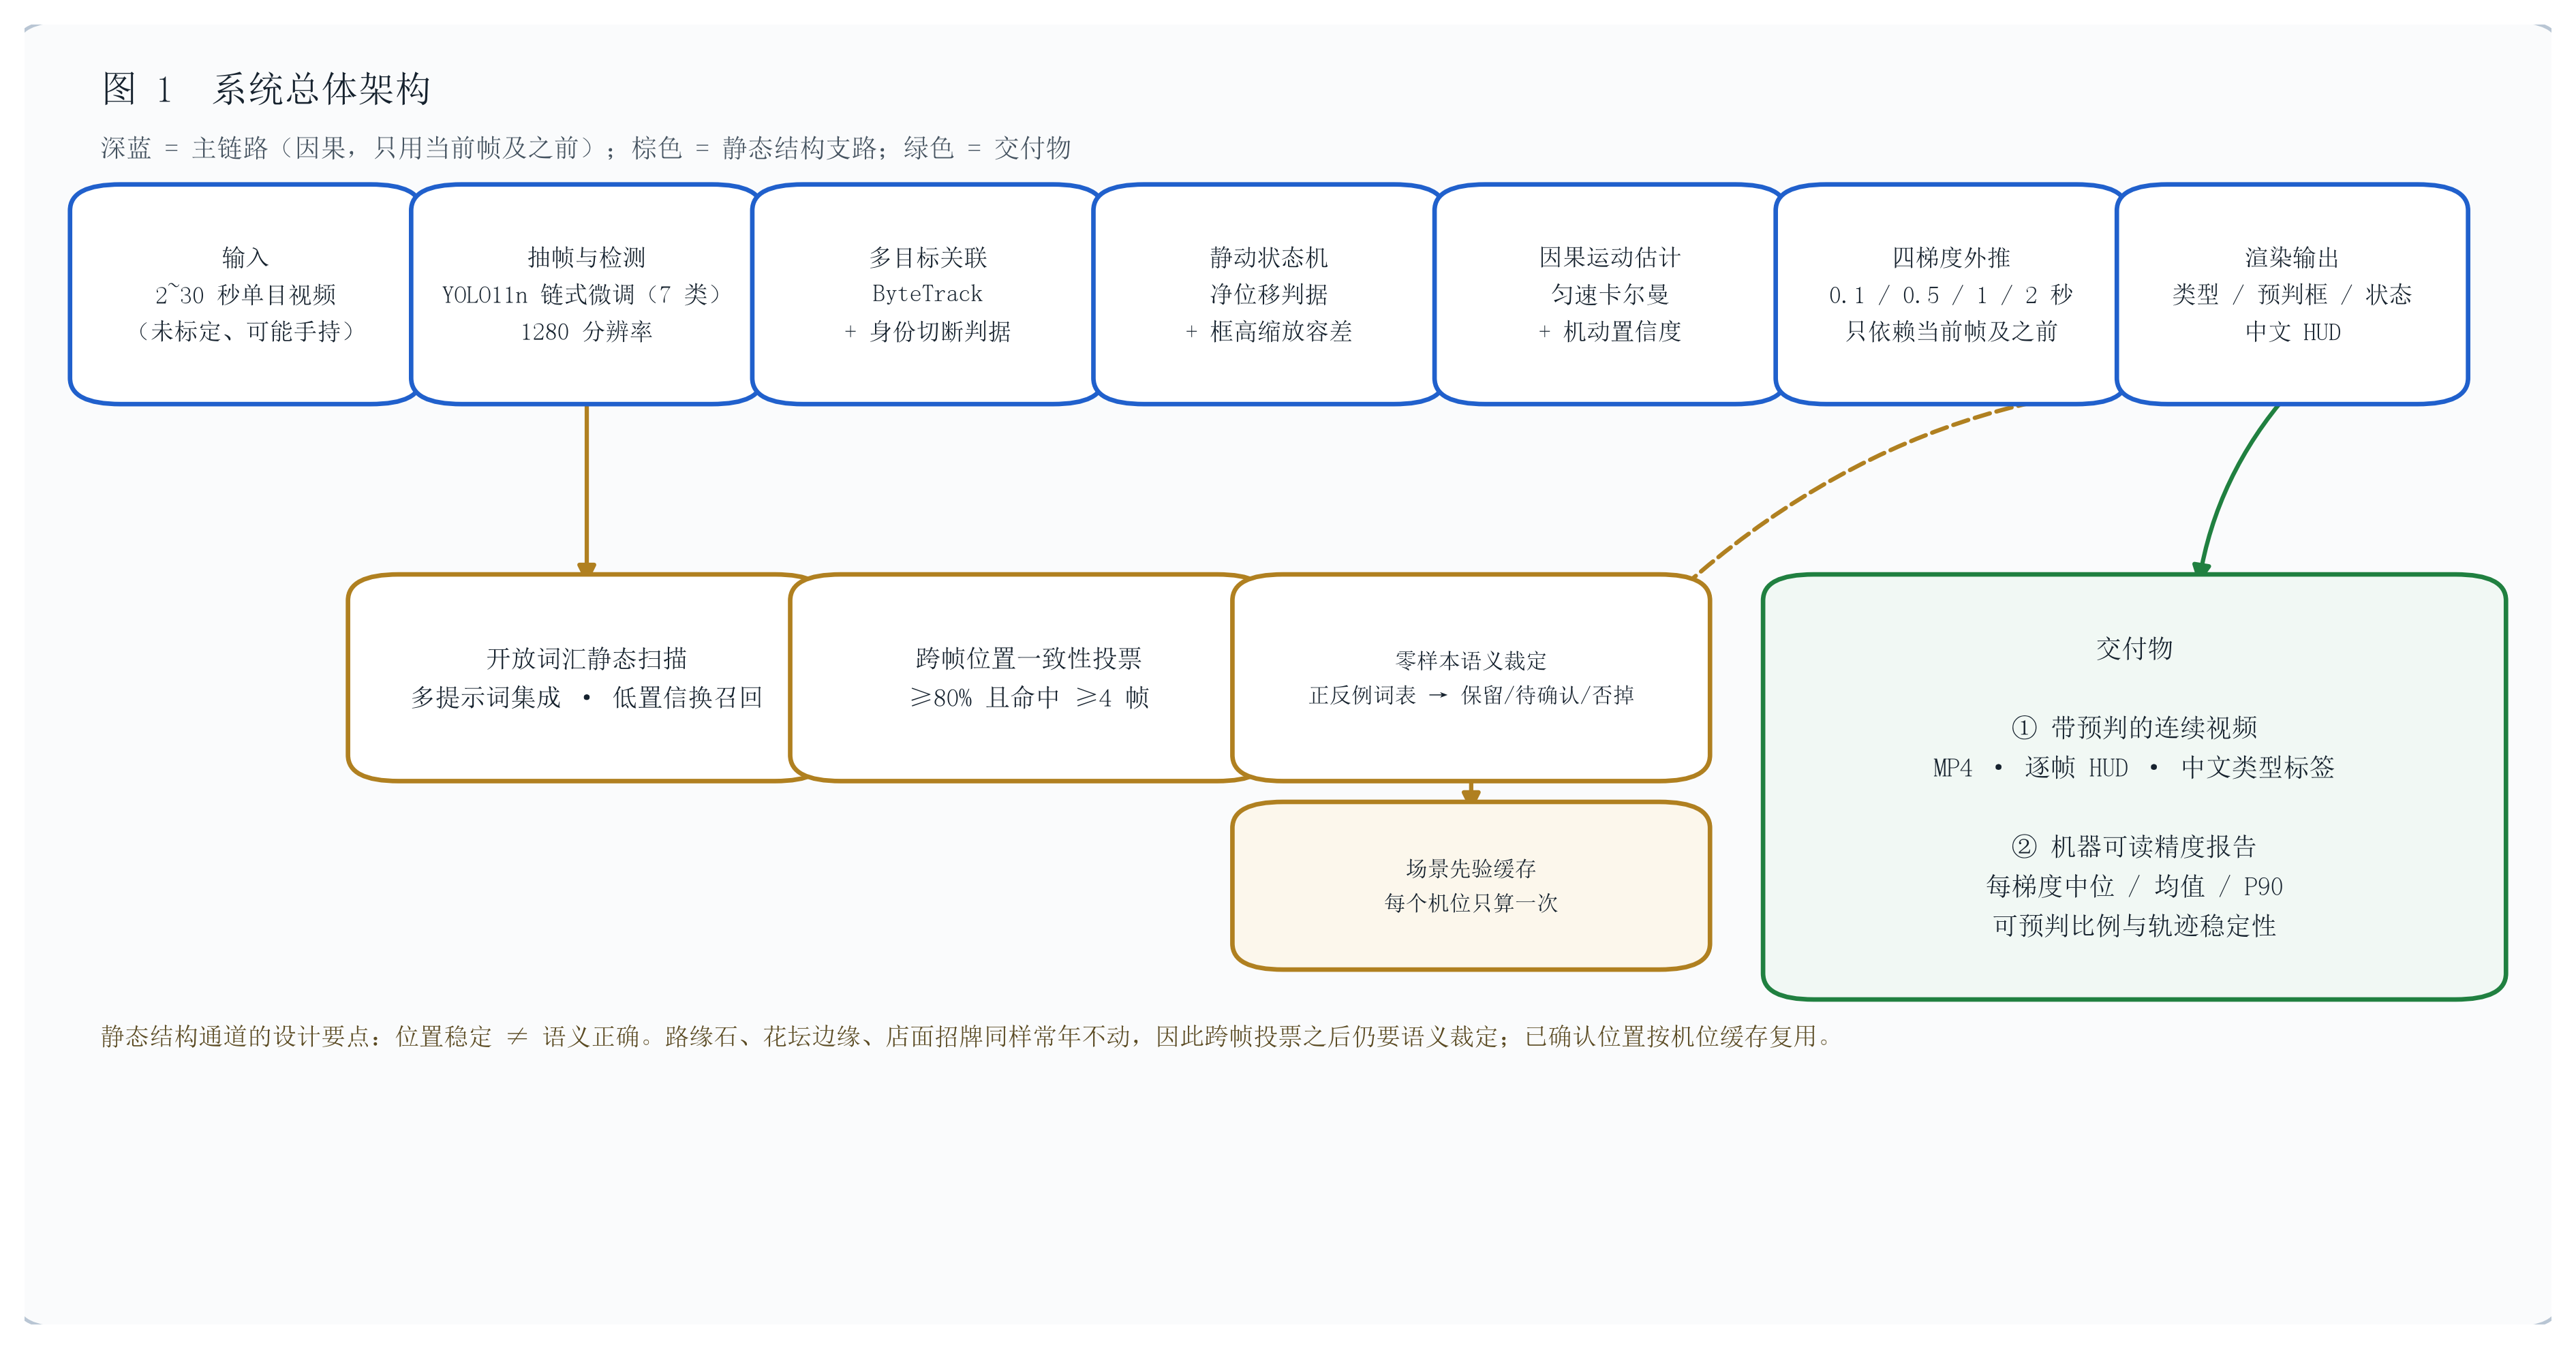
\includegraphics[width=\linewidth]{fig_architecture.png}
\caption{系统总体架构。主链路全程因果，静态结构支路负责固定场景元素的稳定显示。}
\label{fig:arch}
\end{figure}

\subsection{可行性与成本}

全部训练与推理在\emph{单张 8\,GB 消费级笔记本显卡}上完成，不需要服务器或云算力：
共训练 11 个检测版本，累计 438878 秒（约 122 GPU 小时）；推理阶段检测耗时
17$\sim$24\,ms/帧（1280 分辨率），端到端 0.24\,s/帧。这意味着一名学生用一台笔记本
即可完成从数据到交付的全流程，也意味着后续部署不需要专用硬件。

\section{AI 技术与开源及第三方资源选择}

\subsection{AI 在作品中的三类作用}

AI 不是装饰，而是承担三件不可替代的工作：

\textbf{(1) 检测识别}：把像素变成结构化目标。这是全系统唯一的感知入口，
去掉它没有任何低成本的替代方案。

\textbf{(2) 因果外推}：用卡尔曼滤波在含噪观测上维持速度估计，这是"预判"本身。

\textbf{(3) 语义校验}：用零样本图文匹配判断"某个稳定位置到底是什么"。
这一条是本作品的独创用法——它直接回应用户反馈的三类误检（路缘石被当路桩、
广告牌被当标志牌、招牌被当信号灯），而这些误检靠几何或时序规则无法排除。

\subsection{开源资源选型}

关键资源的选型与许可证状态如下（完整清单见附件《开源及第三方资源使用清单》）：

\begin{table}[t]\centering\small
\caption{核心资源的选型、许可证与自研边界。}
\label{tab:res}
\begin{tabular}{p{0.24\linewidth}p{0.17\linewidth}p{0.51\linewidth}}
\toprule
资源 & 许可证 & 使用方式与自研边界 \\
\midrule
ultralytics（检测与跟踪运行时） & AGPL-3.0 & 通过公开 API 调用，未修改上游源码；
其上的预判链路、状态机、串轨防护、静态隐地图、上下文校验全部自研 \\
YOLO 系列预训练权重 & AGPL-3.0 & 作为微调起点；微调得到的 11 个版本权重由团队训练与评测 \\
CLIP（图文匹配） & 元数据标 AGPL-3.0，上游为 MIT &
发行包许可证存在歧义，本作品\emph{按最严（AGPL-3.0）处理}；仅用于静态结构语义校验 \\
filterpy（卡尔曼 / IMM） & MIT & 仅取 IMM 算法做对照实验，\textbf{结论为未采纳} \\
Weighted-Boxes-Fusion & MIT & 用于模型融合对照实验；产品默认未启用 \\
VisDrone（公开数据集） & 原数据集条款 & 仅用于域外泛化验证；\textbf{不再分发原始图像}，只提供转换脚本 \\
\bottomrule
\end{tabular}
\end{table}

\textbf{自研边界声明。}第三方资源提供的是通用能力（检测、跟踪、滤波、数值计算）；
本作品的核心价值——短时预判链路、静态结构稳定性机制、上下文校验、
以及"哪些路线不成立"的系统性实验结论——全部由团队独立完成。

\subsection{一条被评估后放弃的资源}

更强的跟踪器集合（AGPL-3.0）被完整评估后未引入：其内置跟踪器与现有方案同源，
在同一批目标上中位误差只差 1$\sim$3 像素，无收益，却会引入第二条强传染性依赖链。
列出此条是为了说明选型是在许可证与实测收益两方面同时审查过的。

\section{设计与实现过程}

本节只描述四项被团队声明为贡献的设计；其余为常规工程实现。

\subsection{设计一：静态结构隐地图（跨帧投票 + 语义裁定 + 场景先验）}

\textbf{设计。}固定场景元素（路桩、标志牌、路灯、信号灯）会被任何检测器间歇性检出。
分三步建立隐地图：以多提示词集成、低置信度在全片扫描换取召回；按位置跨帧聚簇，
要求"在未被遮挡的帧中至少 80\% 被检出且命中不少于 4 帧"；最后对每个候选外扩
1.8 倍裁出上下文，用零样本图文匹配在正反例词表上打分，输出
\emph{保留} / \emph{待确认} / \emph{否掉} 三档。

\textbf{动机。}时序稳定性只能回答"位置稳不稳"，回答不了"这位置是什么"——
路缘石、花坛边缘、店面招牌同样常年不动，一样能通过一致性检验。实测中，
282 个候选里有 83 个（29\%）被语义裁定否掉，否掉的正是这三类。

\textbf{技术优势。}三点：一是召回优先的扫描 + 投票，使检测器从未学会的路桩
也能稳定显示；二是语义裁定把"看似合规的误检"挡在渲染之前；
三是确认结果按机位缓存为场景先验，使昂贵的扫描与裁定\emph{每个安装点只付一次}
——实测每帧耗时从 318\,ms 降到 81\,ms，且输出逐位一致。

\subsection{设计二：身份切断与带出画判据的遮挡续推}

\textbf{设计。}当目标中心位移超过 $\max(40\,\text{px},\,4\times\text{步长中位})$
\emph{且}与上一帧框重叠低于 0.1 时，判定为串轨，切断轨迹并新建身份；
成熟轨迹被漏检时用卡尔曼外推继续渲染至多 12 帧，且外推中心一旦离开画面立即停止。

\textbf{动机。}实测 7.8\% 的串轨样本贡献了 26\% 的误差总量，中位误差 122 像素，
是最大的单点误差源；而遮挡续推若不加出画判据，会留下"跟着走但画面里没人"的空框
——实测 64\% 的续推目标此后再未被检出。

\textbf{技术优势。}串轨防护把千帧身份跳变从 72.2 降到 43.9（$-39\%$）、涉事轨迹
从 9.1\% 降到 3.5\%；遮挡续推把每帧可预判目标从 10.26 提到 15.84（$+54\%$），
而续推样本自身的中位误差 29.3 像素，并不比实测样本差。

\subsection{设计三：净位移判据的静止状态机}

\textbf{设计。}连续 6 帧未移动的目标判定为静止：不渲染、不预判；重新移动即恢复。
容差随框高缩放；并且在"窗口内波动范围"判据之前先计算\emph{净位移}
（窗口前两帧均值到后两帧均值的距离）。

\textbf{动机。}只看波动范围有一个漏洞：检测框抖动本身会把范围撑大，于是阈值只能放宽，
放宽后走得慢的目标又被当成静止。实测某段第 24 帧 18 条行人里有 14 条被误藏，
其中几条速度是 25$\sim$40\,px/s。净位移上抖动相消、真移动不会，因此它是更可靠的线索。

\textbf{技术优势。}净位移不小于 5 像素时，慢速行人能救回 13.9\%，而停放车辆只有
0.2\% 被误判为运动。同时静态结构类被豁免于隐藏，保证画面中的固定参考物始终可见。

\subsection{设计四：数据集构建与标注规程}

\textbf{设计。}团队自建两套视频数据集（15 段 + 14 段），其中 277 帧、3612 个框由人工
逐帧复核，是本作品唯一的人工真值。规程含三条硬规则：

\emph{先载具、后行人}：骑车、推车与驾驶位上的人只标为载具，骑车人另立类别而不删除
——删除会抹掉"载具有人"这一证据；缺了这条，行人类会被恰好应当按运动载具处理的
那批实例灌水。

\emph{类别序号冻结、只许追加}：前九个序号永不重排，新类一律往后追加，
使类别表扩张时旧标注依然有效（本项目在同一批源标注上并存四套口径）。

\emph{代价不对称，拿不准就留}：漏标对训练模型的伤害远大于误检，
而误检可以在后续专项复核里划掉，删除却无法恢复。

\textbf{动机与优势。}自动预标注不是成品：在同一 277 帧上，人工删除了 14.9\% 的自动框、
补标了 6.5\%（表~\ref{tab:annot}），因此自动标注的残差必须\emph{被测量}而不是被假定。
删除率最高的两类恰好是样本最稀缺的两类，说明自动标注的错误正集中在最需要数据的地方。
复核以离线批次分发（图像目录 + 类别表 + 书面规则 + 零安装浏览器工具，只回传标注），
使复核吞吐不依赖本项目的运行环境。

\begin{table}[t]\centering\small
\caption{标注规程的实测数据（同一 277 帧上自动预标注与人工纠错的逐框比较）。}
\label{tab:annot}
\begin{tabular}{lrlr}
\toprule
统计量 & 数值 & 统计量 & 数值 \\
\midrule
自动产生的框 & 3970 & 静态位置候选 & 282 \\
人工删除 & 592（14.9\%） & \quad 直接保留 & 136 \\
人工补标 & 234（6.5\%） & \quad 送人工确认 & 63 \\
人工改类 & 177 & \quad 语义裁定否掉 & 83（29\%） \\
\quad 卡车类删除率 & 44.8\% & 早期版本的训练/验证泄漏率 & 20.9\% \\
\quad 自行车类删除率 & 40.5\% & \quad（已修正为按视频分段切分） & — \\
\quad 行人删除率 & 25.2\% & & \\
\bottomrule
\end{tabular}
\end{table}

\subsection{生成式 AI 辅助开发的说明}

按赛事要求披露：本作品在开发过程中使用了生成式 AI 辅助，用途与参与环节为
(1) 代码编写与重构（数据预处理、评测脚本、可视化脚本），
(2) 实验结果的统计分析与图表生成，
(3) 文档与本报告的初稿撰写。团队对所有 AI 产出执行了以下审核与验证环节：
每一处引用的数字都必须能由仓库内的可复现脚本复算，且与实验日志逐条核对；
AI 生成的代码在合入前经过实际运行验证（含边界情形）；所有图表由脚本生成而非手工绘制；
方法主张与结论由团队独立判断，AI 不参与结论定稿。AI 生成内容不视为团队的自主知识产权，
本作品主张权利的部分限于第~\ref{sec:innov} 节所列的自研模块与实验结论。

\section{成果展示与效果验证}

\subsection{系统实际输出}

图~\ref{fig:sample} 是系统的真实输出画面：左上为运行状态（预判梯度、帧号、
跟踪目标数与静态记忆数），画面中实线框为当前检测（含类型与跟踪 ID），
虚线框为预判位置，"遮挡续推"标记被遮挡仍在显示的轨迹，
"路灯·记忆/信号灯·记忆/路桩·记忆"为静态结构隐地图补回的固定结构。

\begin{figure}[t]\centering
\includegraphics[width=\linewidth]{fig_output_annotated.png}
\caption{系统实际输出画面（真实运行结果的单帧，未做修饰）与框线样式图例。}
\label{fig:sample}
\end{figure}

\subsection{检测端结果}

\begin{table}[t]\centering\small
\caption{检测精度（mAP50\up，输入分辨率 1280）。}
\label{tab:det}
\begin{tabular}{lccc}
\toprule
验证集 & 链式微调 7 类 & 从零训练 nano & 从零训练 small \\
\midrule
目标域（65 帧） & \textbf{0.637} & 0.615 & 0.597 \\
旧街面（116 帧） & \textbf{0.701} & 0.636 & 0.698 \\
航拍域外（399 帧） & 0.407 & 0.310 & \textbf{0.408} \\
\bottomrule
\end{tabular}
\end{table}

两点结论：\textbf{训练历史比模型容量更重要}——同配方从零训练的 nano 只有 0.615，
低于链式微调的 0.637；\textbf{换更大骨干没有赢}——small 骨干精确率更高（0.673 对
0.604）但召回低 23\%（0.479 对 0.620）。模型融合可把目标域提到 0.634，
代价是推理成本翻倍且牺牲实时性，因此产品默认未切换。

\subsection{预判端主结果与组件消融}

\begin{table}[t]\centering\small
\caption{规范预判口径下的主结果。协议：六段各 300 帧、置信度 0.25、分辨率 1280、
关闭静态通道、已修正 NMS。}
\label{tab:main}
\begin{tabular}{lrrrr}
\toprule
梯度 & 样本数 & 误差中位 (px)\dn & 沿运动方向有符号误差中位 (px) & 滞后占比 \\
\midrule
0.1\,s & 16635 & 3.8 & $-0.8$ & 41.7\% \\
0.5\,s & 13125 & 14.3 & $-6.5$ & 34.6\% \\
1.0\,s & 10004 & 30.5 & $-15.6$ & 34.2\% \\
2.0\,s & 6248 & 67.3 & $-36.9$ & 32.0\% \\
\midrule
每帧目标数 & \multicolumn{4}{r}{33.3} \\
每帧可预判目标数 & \multicolumn{4}{r}{14.87（占检出 44.6\%）} \\
1 秒中位误差（各段范围） & \multicolumn{4}{r}{26.6$\sim$49.5\,px} \\
轨迹跳变 & \multicolumn{4}{r}{18.3 次/千帧} \\
\bottomrule
\end{tabular}
\end{table}

四项组件消融各自改变了不同环节：身份切断使千帧跳变 72.2$\rightarrow$43.9；
遮挡续推使每帧可预判 10.26$\rightarrow$15.84；分辨率 960$\rightarrow$1280 使目标域
mAP50 0.585$\rightarrow$0.637、精确率 0.459$\rightarrow$0.604；
场景先验缓存使每帧 318\,ms$\rightarrow$81\,ms。

\subsection{误差结构：本作品的核心实测发现}

本节是本作品区别于"做完跟踪就交差"的关键——我们把预判误差本身当作研究对象。

\textbf{发现一：误差几乎全部沿运动方向，且以系统性超调为主。}
垂直方向误差的中位数在所有类别、所有梯度上都在 $\pm0.4$ 像素以内；
而沿运动方向的中位偏差随梯度从 $-0.8$ 增长到 $-36.9$ 像素，且只有 32\%$\sim$42\%
的样本滞后（图~\ref{fig:signed}）。这意味着方向环节没有系统性缺陷，
问题出在量级上：全局位移增益即使取最优（0.92），平均绝对误差也只改善 2.5\%。

\begin{figure}[t]\centering
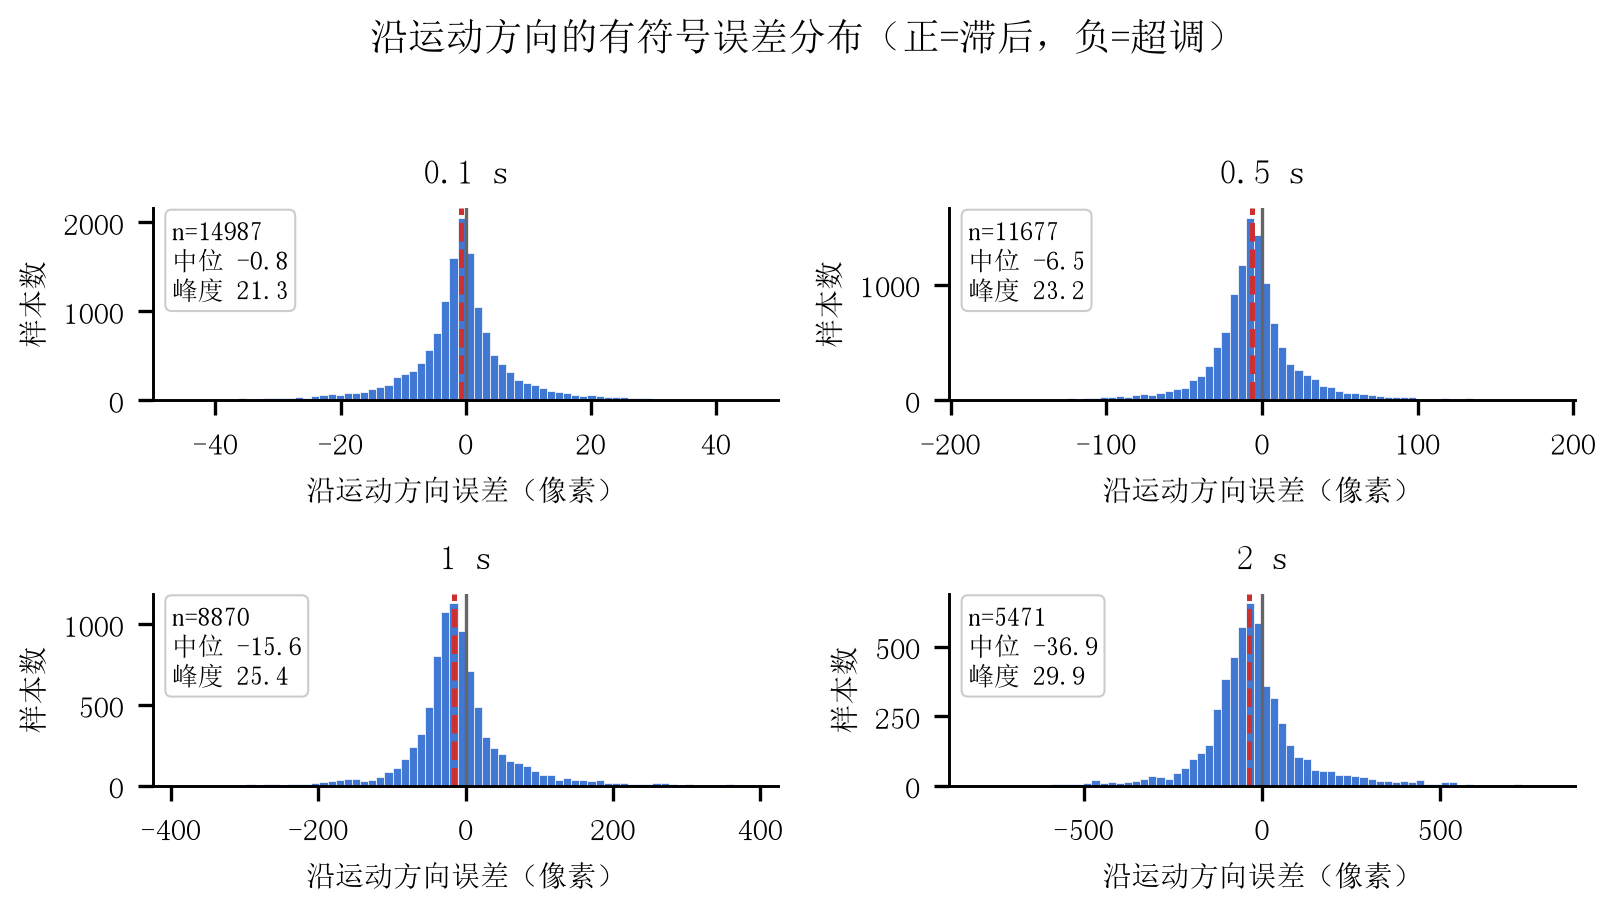
\includegraphics[width=\linewidth]{fig_signed_error.png}
\caption{各梯度沿运动方向的有符号误差分布（正=滞后，负=超调）。}
\label{fig:signed}
\end{figure}

\textbf{发现二：误差分布是尺度混合，不是任何单一分布族。}
误差幅值分布的峰度达 21$\sim$30、均值/中位为 1.76$\sim$1.81，明显非高斯。
进一步把七个分布族放在 24 个"类别 $\times$ 梯度"单元格上横评：
带折点的两片高斯与偏正态\textbf{一次都没赢过}，稳定胜出的是学生 $t$ 与两成分高斯混合
——两者都是\emph{尺度混合}。拟合结果：约 21\%$\sim$36\% 的样本来自一个宽度为主体
3$\sim$8 倍的分量，却贡献了 \textbf{75\%$\sim$98\% 的总方差}（图~\ref{fig:mix}）。

\begin{figure}[t]\centering
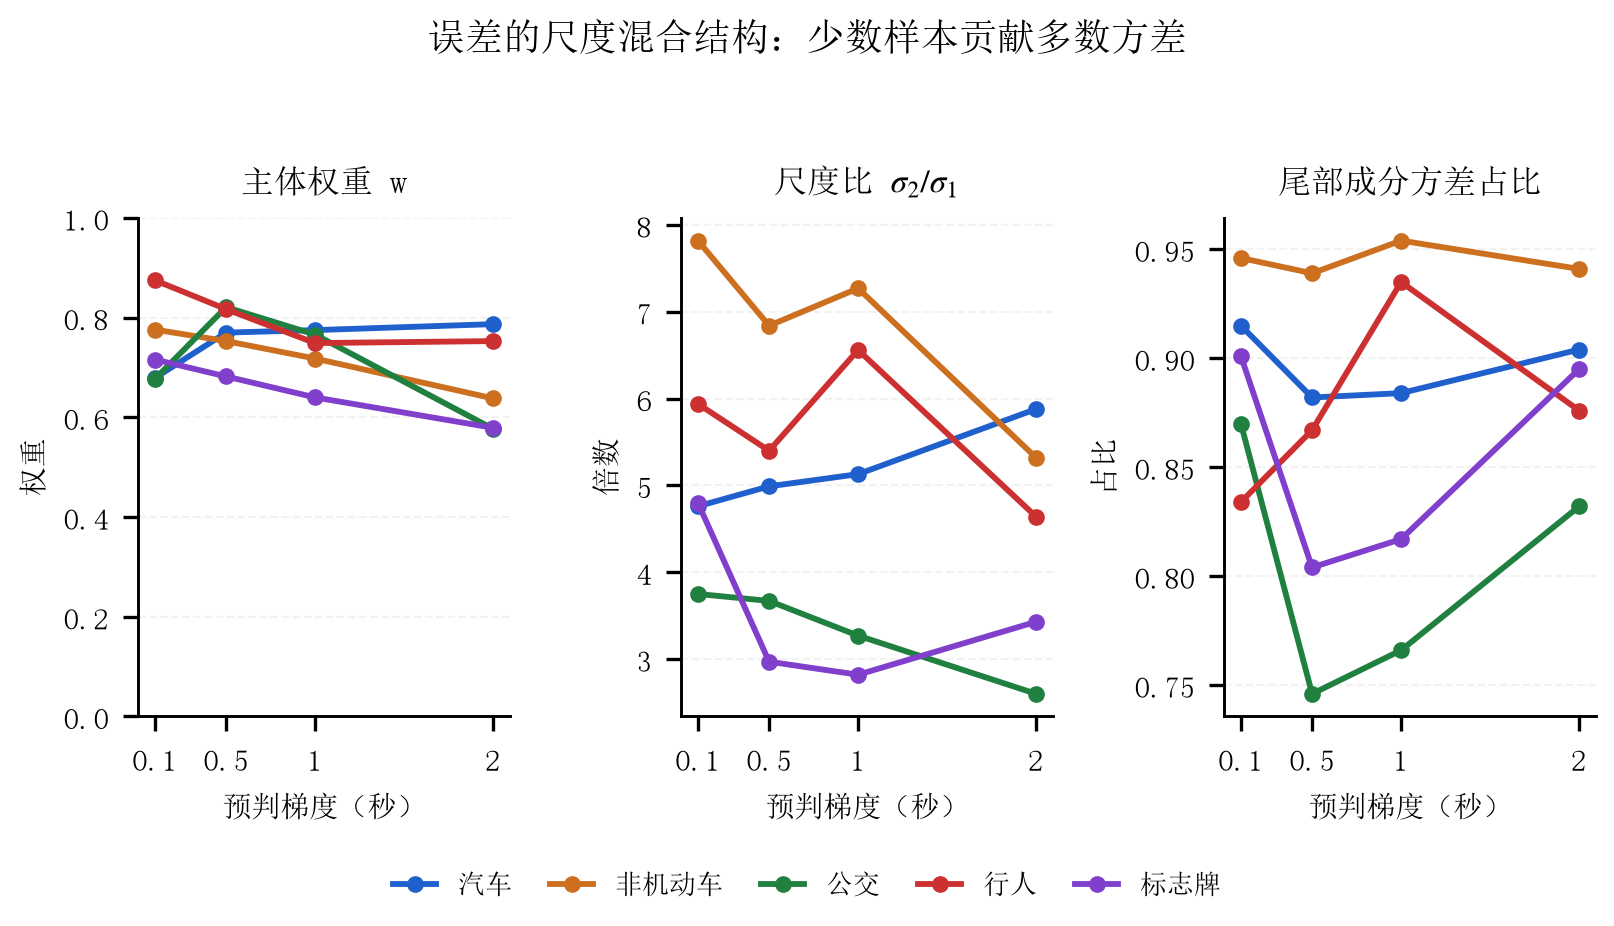
\includegraphics[width=\linewidth]{fig_scale_mixture.png}
\caption{尺度混合的三个判据量随梯度的走向：主体权重、尺度比、尾部分量方差占比。
卡车类因样本量不足（619 个）未纳入本图。}
\label{fig:mix}
\end{figure}

\textbf{发现三：重尾不是透视尺度造成的假象。}
把误差除以框高（预测时刻已知、且透视下像素位移与目标像素尺寸成正比）后，
对数误差与对数框高的相关系数只有 0.192，框高仅解释 3.7\% 的方差；
两类口径判定的重尾样本只有 12.5\% 不一致；即使把全部尺度代理特征从因果门控中剔除，
样本外曲线下面积仍有 0.714（图~\ref{fig:scalecontrol}）。
这排除了"重尾只是近处目标像素大"这一最自然的怀疑。

\begin{figure}[t]\centering
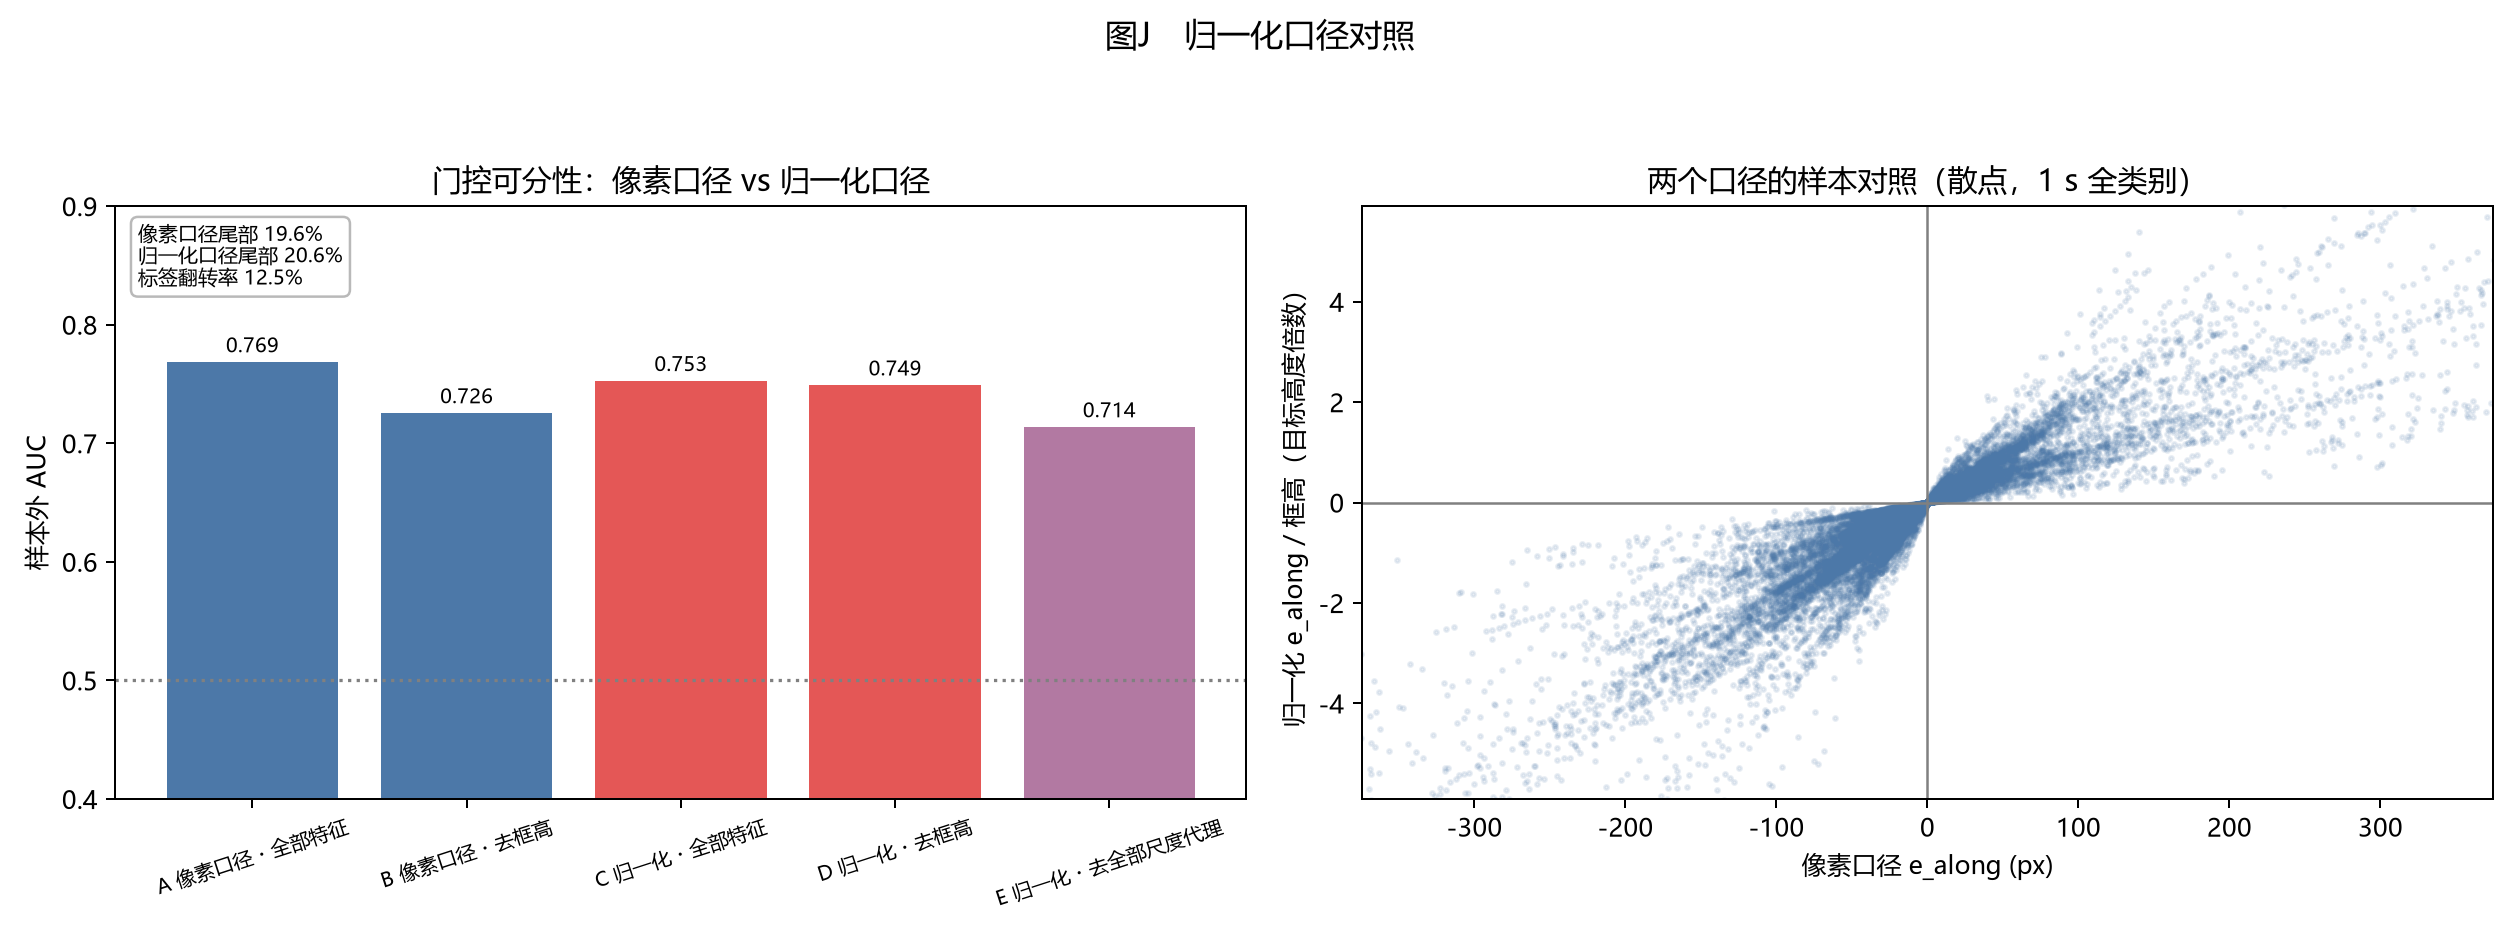
\includegraphics[width=\linewidth]{fig_scale_control.png}
\caption{尺度归一化对照：五个特征变体的样本外可分性与两口径散点对比。}
\label{fig:scalecontrol}
\end{figure}

\textbf{发现四：误差质量集中在少数类别，机制修复的收益有明确上限。}
像素口径下，汽车占误差总量的 68.5\%、非机动车占 17.8\%，而静态结构只占 1.6\%；
各类别的\emph{单位样本}均值其实接近（28$\sim$41 像素），总量差全在样本数上。
据此解析评估"静态结构零位移预判"（预判框=当前框）：标志牌 1 秒档中位从 31.9 降到
9.5 像素（$-70\%$）、2 秒档从 64.3 降到 10.6（$-84\%$），但折算到全体只有
\textbf{$-1.0\%$} 的误差总量（图~\ref{fig:attrib}）。结论是：\emph{值得做，
局部收益巨大且零成本，但改不了大局}。

\begin{figure}[t]\centering
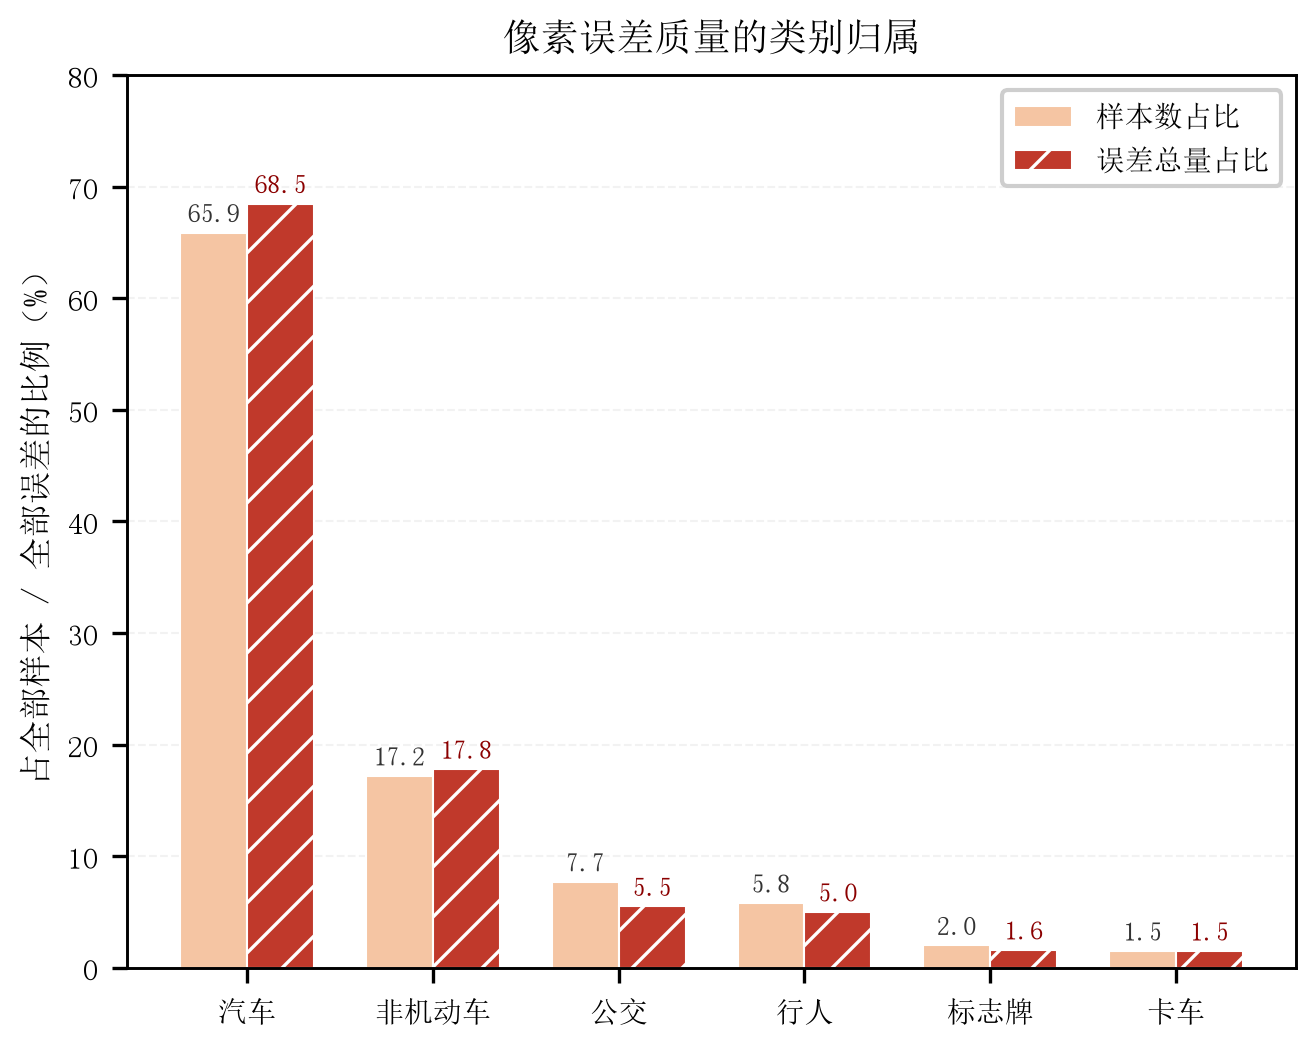
\includegraphics[width=\linewidth]{fig_error_attribution.png}
\caption{像素口径下的误差质量归属与静态结构零位移预判的局部收益。}
\label{fig:attrib}
\end{figure}

\begin{figure}[t]\centering
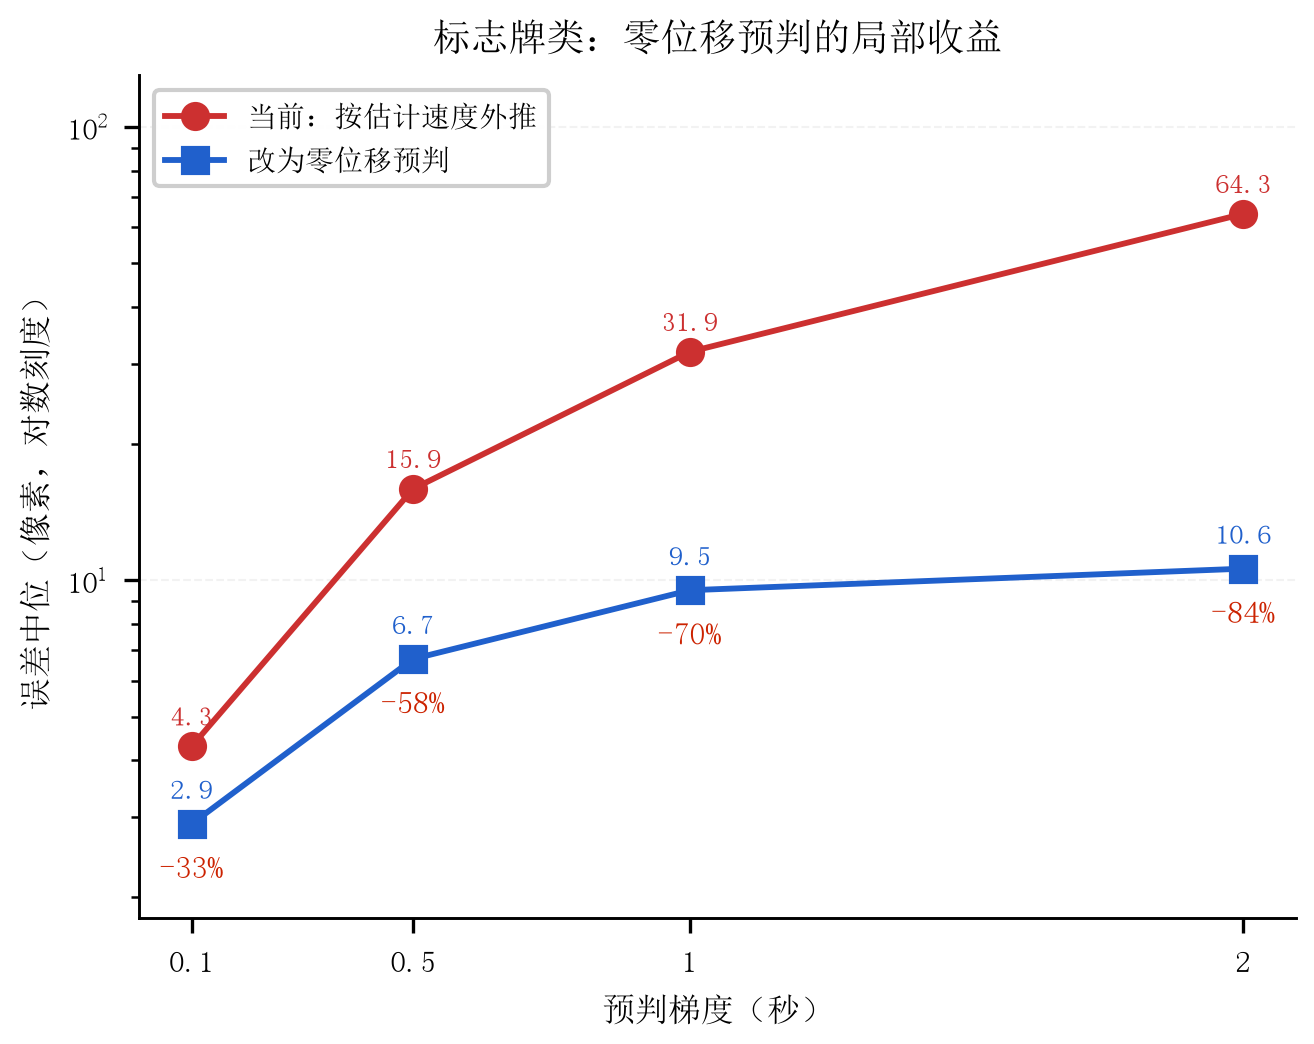
\includegraphics[width=0.78\linewidth]{fig_static_fix.png}
\caption{静态结构类改为零位移预判后，标志牌在四个梯度上的中位误差变化（对数纵轴）。}
\label{fig:static}
\end{figure}

\subsection{负结果：已实测否掉的十二族方案}

\begin{table}[t]\centering\small
\caption{已被实测否掉的技术路线（同一评测协议下）。}
\label{tab:neg}
\begin{tabular}{p{0.30\linewidth}p{0.62\linewidth}}
\toprule
路线 & 实测结果 \\
\midrule
匀加速外推 & 比匀速差 3$\sim$8 倍 \\
圆弧外推（CTRV） & 阻尼转角扫描中 gain$=0$ 在每一档最优 \\
交互式多模型（IMM） & 8573 配对样本中仅 50\% 更准，中位/均值/P90 全面略差 \\
自适应卡尔曼 & P90 从 116.6 恶化到 125.8 \\
地面平面逆透视（BEV） & 中位 34.6$\rightarrow$45.9、均值 57.7$\rightarrow$167.1 \\
切图推理 & 目标域 0.615$\rightarrow$0.600 \\
输入分辨率 1600 & 劣于 1280 \\
更大骨干（small） & 目标域 0.597 对 0.637，召回低 23\% \\
更换跟踪器（BoT-SORT / OC-SORT） & 同批目标中位误差仅差 1$\sim$3 像素 \\
长关联缓冲 & 可预判升至 12.11/帧，但跳变从 72 翻倍到 149 次/千帧 \\
事后门控筛选重尾样本 & 像素口径下的收益来自筛掉近处大目标；换尺度无关标签后无收益甚至有害 \\
全局位移增益校正 & 平均绝对误差仅改善 2.5\% \\
\bottomrule
\end{tabular}
\end{table}

\subsection{面向在线部署的实测可行性}
\label{sec:stream}

我们对"能否走向在线分析"做了实测而非估计。统一条件：每配置消耗 600 个源帧、
输入分辨率 1280、关闭渲染与 JSON 导出（只计分析路径）。检测采用\textbf{跳帧}
——每 $N$ 帧抽 1 帧检测，中间帧在容器层掠过（只解复用、不解码），时间戳仍取自
容器，因此运动模型的时间步长与实际间隔一致。

\begin{table}[t]\centering\small
\caption{跳帧带来的流效率（每配置消耗 600 个源帧）。30\,fps 素材需要 33.3 毫秒/帧，
故等效源帧率 33 以上即越过实时线。毫秒每源帧越低越好\dn，等效源帧率越高越好\up。}
\label{tab:stream}
\begin{tabular}{lrr}
\toprule
配置 & 毫秒 / 源帧\dn & 等效源帧率\up \\
\midrule
stride 1（基线）· 1280 & 48.2 & 20.8 \\
stride 2 · 1280 & \textbf{29.1} & \textbf{34.4} \\
stride 3 · 1280 & \textbf{23.2} & \textbf{43.1} \\
stride 1 · 736（720p 档） & 44.8 & 22.3 \\
stride 3 · 736（720p 档） & 22.1 & 45.4 \\
\midrule
完整离线路径（渲染 + 导出）· stride 1 · 1280 & 69.2 & 14.4 \\
\bottomrule
\end{tabular}
\end{table}

\textbf{结论一：跳帧一步即越过 30\,fps 实时线。}stride 2 达到 34.4 等效源帧率，
stride 3 达到 43.1。需要说明，此前记录的"端到端 0.24\,s/帧"是\emph{未命中场景先验
缓存}时的旧口径；命中缓存后完整离线路径只需 69.2 毫秒/帧，而在线化并不需要渲染
与导出，分析路径本身仅 48.2 毫秒/帧。

\textbf{结论二：降分辨率基本不值。}同一 stride 下，736 只比 1280 快 5\%$\sim$7\%，
精度代价却是 10\%。因此在线化的正确方向是\textbf{跳帧}，不是降分辨率，
更不是换更大的骨干（后者已被实测否掉，表\ref{tab:neg}）。

\textbf{结论三（反直觉，经三段视频复验）：跳帧不损失精度，反而普遍更好。}
为排除评估口径的干扰，这里把真值\textbf{固定为 stride=1 的稠密观测}，只让预判来自
不同 stride 的运行。由于跟踪器在每次运行时自行分配目标 ID、两次运行的 ID 不可比，
稀疏预测通过"同一时刻、同类别、中心最近"的空间匹配挂到稠密轨迹上
（阈值 15 像素，漏配率 0.5\%$\sim$1.5\%）。

\begin{table}[t]\centering\small
\caption{真值固定为 stride=1 稠密观测时的精度对照（三段视频，各 600 源帧）。
1 秒档给出三种 stride 的中位误差，括号内为相对基线的变化；2 秒档只列基线与
stride 3 以节省版面。误差越低越好\dn。}
\label{tab:stride-acc}
\begin{tabular}{lrrrrr}
\toprule
片段 & \multicolumn{3}{c}{1 秒档中位 (px)\dn} & \multicolumn{2}{c}{2 秒档中位 (px)\dn} \\
\cmidrule(lr){2-4}\cmidrule(lr){5-6}
 & stride 1 & stride 2 & stride 3 & stride 1 & stride 3 \\
\midrule
片段一 & 23.3 & 21.7（$-6.9\%$） & 20.9（$-10.3\%$） & 62.5 & 61.5 \\
片段二 & 28.6 & 18.4（$-35.7\%$） & 14.8（$-48.3\%$） & 61.7 & 26.7 \\
片段三 & 38.2 & 33.8（$-11.5\%$） & 31.7（$-17.0\%$） & 60.8 & 33.9 \\
\bottomrule
\end{tabular}
\end{table}

三段视频上跳帧都\emph{没有}损失精度，且 1 秒与 2 秒档普遍更好，2 秒档改善最大。
机制上讲得通：30\,fps 下相邻帧的目标中心位移很小，速度估计被检测抖动主导；
抽到 10\,fps 后每步位移变为三倍，速度估计的信噪比按比例改善。这与本报告前面
"误差主要由像素位移速度决定"的实测一致。由于三个配置\emph{共用同一份真值}，
该比较在相对意义上是成立的。

\textbf{仍缺的部分是工程而非算法。}当前系统是无状态批处理器：每个视频从零加载模型、
重扫静态结构、结束即退出。真正在线化需要常驻进程、模型只加载一次、
每个机位扫描一次后长期复用场景先验、流式接收帧并把结果推给前端。
本作品\emph{未}包含这部分对接；按上述实测，算法侧已不再构成瓶颈。

\section{创新性与开放价值}
\label{sec:innov}

\subsection{创新点}

\textbf{创新点一：静态结构的两段式判定（位置一致性 + 语义裁定）。}
现有做法要么依赖检测器直接检出，要么只用时序一致性投票。本作品指出并实测证明了
后者的不足——29\% 的稳定候选其实是路缘石、花坛边缘与店面招牌；
并用零样本图文匹配补上"这位置是什么"这一步，配合出画判据与场景先验缓存，
把固定结构的误检与闪烁同时解决。

\textbf{创新点二：误差分布的尺度混合刻画。}本作品不停留在报平均误差，
而是把预判误差当作随机变量逐层拟合分布族，证明它是尺度混合而非单一分布，
并给出两个可直接使用的判据量（主体权重 $w$、尺度比 $\sigma_2/\sigma_1$）。
该刻画解释了此前分散的多个现象：为什么全局增益不值钱、为什么带折点的模型全败、
为什么尾部风险与均值风险需要分开对待。

\textbf{创新点三：系统性的负结果地图。}十二族方案被逐一实现并实测否掉，
形成一张可复用的"不要再试"清单。在短时单目预判这个方向上，
这比再提出一个略优的模型对后来者更有价值。

\subsection{开放成果与复用价值}

\begin{itemize}\setlength{\itemsep}{1pt}
  \item \textbf{代码与工具}：预判软件本体、静态隐地图、上下文校验、88 个评测脚本、
        中文标注复核工具，整体以 AGPL-3.0 开放；
  \item \textbf{数据工具}：标注规程文档、离线批次分发与回收脚本、
        自动标注质量评估脚本（可复用于其他交通视频数据集建设）；
  \item \textbf{评测资产}：12 条负结果的完整实验记录与可复现脚本；
  \item \textbf{文档}：方法说明、复现说明、资源与许可证清单。
\end{itemize}

权利边界清晰：第三方资源提供通用能力，自研部分的边界在第~\ref{sec:innov} 节与
第三章中逐条列明。维护计划为：模型与评测脚本随数据集扩充持续更新；
标注工具与批次分发脚本保持独立可用，不依赖本项目的运行环境。

\section{合规、安全与风险说明}

\textbf{许可证核验。}全部 Python 依赖的许可证已逐一读取发行包元数据或包内
\texttt{LICENSE} 原文，不存在"公开可访问即视为可自由使用"的假设。
其中 \texttt{clip} 发行包的元数据与包内许可证冲突，本作品\emph{按最严（AGPL-3.0）}处理。

\textbf{AGPL 的处置决定。}检测与关联链路的强传染性决定了本作品整体以 AGPL-3.0 开放
发布——该链条无法通过闭源规避，而开放发布同时满足合规要求与"开放成果"这一评分维度。
若后续需要闭源交付，替代路径为：检测换用 Apache-2.0 许可的实现，跟踪按公开论文自研；
该路径已做过可行性评估，属工程工作量而非研究风险。

\textbf{数据与隐私。}自采视频含公众场景，公开前须完成人脸与车牌脱敏（当前状态：待完成）；
第三方航拍数据只提供转换脚本，不再分发原始图像。

\textbf{风险与能力边界。}三条必须如实说明：
(1) 本作品全部预判数字的真值取自\emph{同一跟踪器的未来观测}，衡量的是自洽性而非绝对
正确性，因此结论应被理解为结构性的（误差长什么样、错在哪一侧、哪些路线无效）；
(2) 人工真值仅 277 帧，分类型结论在卡车（619 样本）与标志牌（813 样本）上不稳定；
(3) 极小的目标（短边不足 8 像素）被策略性放弃，不识别也不预判。

\section{总结与展望}

\textbf{总结。}本作品交付了一套可在单张 8\,GB 显卡上运行的单目交通视频短时预判软件，
规范口径下目标域检测 mAP50 0.637、每帧可预判 14.87 个目标、1 秒预判中位误差 33.4 像素。
更重要的是给出了三项可复用的认识：静态结构需要位置与语义两段式判定；
预判误差是尺度混合而非单一分布，少数样本贡献绝大多数方差；
短时单目预判的算法收益已接近枯竭，十二族替代方案被实测否掉。

\textbf{展望。}下一步有两条尚未被证否的路径。
其一，\textbf{数据}：用独立人工真值替换自证式真值，并补齐非机动车（贡献 17.8\% 误差量
却只有 7033 样本）与卡车（619 样本）的标注。
其二，\textbf{标定}：固定机位下一次相机标定即可把像素预判换算为米与千米每小时，
并解锁此前被否掉的地面平面建模——这是唯一\emph{新增}输出而非改善已有输出的改动，
也是本作品从"框画得更准"走向"输出可直接用于限速与冲突预警的物理量"的关键一步。
在部署形态上，第~\ref{sec:stream}~节的实测表明算法侧已可越过 30\,fps 实时线（跳帧 stride 2 达到
34.4 等效源帧率且不损失精度），剩余工作是把它由无状态批处理器改造为常驻服务。

\appendix
\section{复现方式与运行环境}

\begin{itemize}\setlength{\itemsep}{1pt}
  \item 运行环境：Windows + Python 3.11 + PyTorch（CUDA 12.8+）+ ultralytics；
        无需服务器，单张 8\,GB 显卡即可。
  \item 预判出视频：
        \texttt{python -m trafficvision.cli --video 输入.mp4 --horizon 1 --out 输出.mp4}
        （四个梯度取 0.1 / 0.5 / 1 / 2；同机位多段视频加 \texttt{--camera <机位名>}
        可复用场景先验）。
  \item 精度报告：同一命令加 \texttt{--json 报告.json}，输出逐帧目标与逐梯度指标。
  \item 复现主结果：\texttt{python bench/run\_predict\_set.py}（六段各 300 帧，规范口径）。
  \item 复现误差结构分析：\texttt{python bench/error\_distribution.py}。
  \item 复现演示视频：\texttt{python bench/make\_demo\_video.py}。
\end{itemize}

\section{附件与参考}

\begin{itemize}\setlength{\itemsep}{1pt}
  \item 附件：《开源及第三方资源使用清单》（含资源名称、版本/来源、许可证、
        使用方式、关键许可义务、自主开发边界与合规状态）。
  \item 演示视频：\texttt{trafficvision\_demo.mp4}（H.264，1920$\times$1080，
        3 分 34 秒，68.5\,MB，全部画面为真实运行输出）。
  \item 参考文献 40 条（含匀速基线的原始研究、跟踪与检测的原始论文、
        以及被否掉路线的对应文献），已逐条核对编号与出处。
\end{itemize}

\end{document}
